\documentclass[a4paper,12pt]{article} 
\usepackage{baseset}
\DeclareSymbolFont{operators}{OT1}{ntxtlf}{m}{n}
\SetSymbolFont{operators}{bold}{OT1}{ntxtlf}{b}{n}
\usepackage{wasysym}
\usepackage{multirow}
\graphicspath{{images/}}
\DeclareGraphicsExtensions{.pdf,.png,.jpg}
\usepackage{subfigure}

%Заговолок
\author{Красоткина Виктория}

\title{Лабораторная работа 1.2.5

Исследование вынужденной регулярной прецессии гироскопа}

\date{24 октября 2022 г.}

\begin{document}

\maketitle
\thispagestyle{empty}

\newpage
\setcounter{page}{1}

	\textbf{Цель:} исследовать вынужденную прецессию гироскопа; установить зависимость скорости вынужденной прецессии гироскопа от величины момента сил, действующих на ось гироскопа; определить скорость вращения ротора гироскопа и сравнить ее со скоростью, рассчитанной по скорости прецессии.
	
	\textbf{Приборы:} 
	\begin{itemize}
		\item гироскоп в кардановом подвесе
		\item секундомер
		\item набор грузов
		\item отдельный ротор гироскопа
		\item цилиндр известной массы,
		\item крутильный маятник
		\item штангенциркуль
		\item линейка
	\end{itemize}


\subsection*{Теоретическая часть}

Основные уравнения движения твердого тела можно записать в виде:

\begin{equation}
	\frac{d\vec{P}}{dt} = \vec{F}
	\label{eq:center_of_mass}
\end{equation}

\begin{equation}
	\frac{d\vec{L}}{dt} = \vec{M}
	\label{eq:moments_equation}
\end{equation}

Формула (\ref{eq:center_of_mass}) выражает закон движения центра масс, а формула (\ref{eq:moments_equation}) -- уравнение моментов, действующих на тело. Двух данных уравнений достаточно для описания состояния твердого тела.

Если сила $\vec{F}$ не зависит от угловой скорости вращения тела, а момент $\vec{M}$ от скорости поступательного движения тела, то уравнения (\ref{eq:center_of_mass}) и (\ref{eq:moments_equation}) можно рассматривать независимо друг от друга. В данной работе рассматривается только задача о вращении твердого тела.

Момент импульса твердого тела можно вычислить, используя формулу:
\begin{equation}
	\vec{L} = \vec{i}I_{x}\omega_{x} + \vec{j}I_{y}\omega_{y} + \vec{k}I_{z}\omega_{z},
\end{equation}
где $ I_{x},I_{y},I_{z} $ -- главные моменты инерции тела, $ \omega_{x}, \omega_{y}, \omega_{z} $ -- компоненты вектора угловой скорости  $\vec{\omega} $.

Быстро вращающееся тело, для которого:

	$$I_{z}\omega_{z} \gg I_{x}\omega_{x}, I_{y}\omega_{y}$$

принято называть \textit{гироскопом}. Гироскоп называется уравновешенным, если его центр масс неподвижен.

В силу (\ref{eq:moments_equation}), приращение момента импулься определяется интегралом:
\begin{equation}
	\Delta\vec{L} =  \int\vec{M}\\,dt
	\label{eq:integral_for_increment}
\end{equation}

Если момент внешних сил действует в течение короткого промежутка времени, из формулы (\ref{eq:integral_for_increment}) следует, что приращение $\vec{L}$ момента импулься значительно меньше самого момента импульса, т.е:

$$
	\left| \Delta\vec{L} \right| \ll \left| \vec{L} \right|.
$$

Благодаря этому, гироскоп приобретает очень большую устойчивость, вызванную его быстрым вращением.

Если гироскоп уравновешен, то суммарный момент сил, действующих на него, равен 0. В таком случае, гироскоп не будет изменять своего положения в пространстве. Если на гироскоп в течение длительного времени будет действовать некоторый момент сил, отличный от нуля, то, согласно (\ref{eq:moments_equation}) гироскоп придет в движение. Мы не будем рассматривать действие моментов сил, которые вызовут ускорение или замедление гироскопа (т.е. моментов сил, которые не изменяют положения оси вращения гироскопа). Рассмотрим действия моментов сил, которые изменяют положение оси вращения гироскопа.

\begin{wrapfigure}[19]{r}{0.4\textwidth}
	\vspace{-2.5ex}
	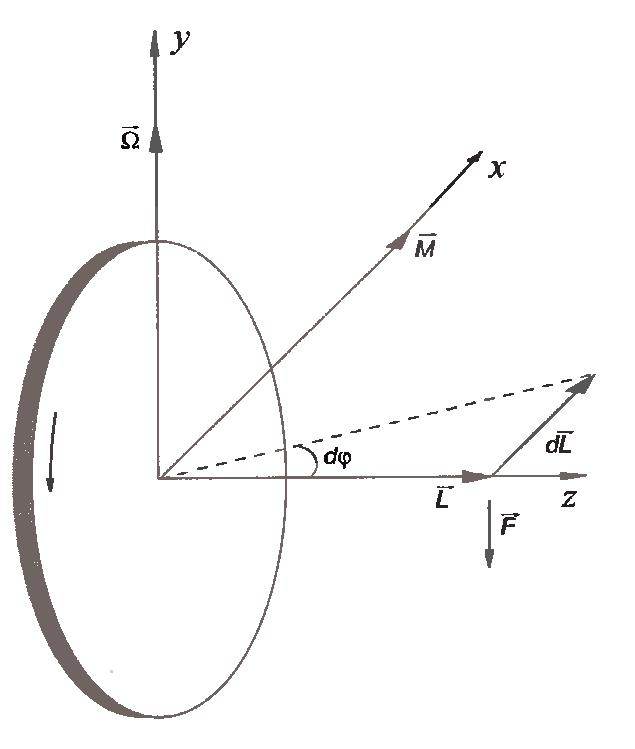
\includegraphics[width = 0.35\textwidth]{flywheel}
	\caption{Маховик.}
	\label{fig:flywheel}
\end{wrapfigure}

Рассмотрим маховик, вращающийся вокруг оси z. (Рис. \ref{fig:flywheel}). Будем считать, что 
$$ \omega_{z} = \omega_{0},\qquad \omega_{x} = \omega_{y} = 0.$$

Пусть ось вращения повернулась в плоскости \textit{zx} по направлению в оси \textit{x} на бесконечно малый угол $d\varphi$. Такой поворот означает добавочное вращение маховика вокруг оси \textit{y}, так что 
$$ d\varphi = \Omega\,dt, $$
где $ \Omega $ -- угловая скорость такого вращения. Будем предполагать, что
\begin{equation}
	L_{\Omega} \ll L_{\omega_{0}}
	\label{eq:condition_for_rotate}
\end{equation}

Это означает, что момент импульса маховика, равный $I_{z}\omega_{0}$ до приложения внешних сил, только повернется в плоскости \textit{zx} по направлению к оси \textit{x} не изменяя своей величины. Таким образом,

\begin{equation}
	\left|d\vec{L}\right| = Ld\varphi = I\Omega\,dt
	\label{eq:increment_moment_of_impulse}
\end{equation}


Записывая выражение (\ref{eq:increment_moment_of_impulse}) в виде векторного произведения, получаем:

$$
	\frac{d\vec{L}}{dt} = \vec{\Omega} \times \vec{L}
$$

Окончательно, используя (\ref{eq:moments_equation}), получаем:

\begin{equation}
	\vec{M} = \vec{\Omega} \times \vec{L}
	\label{eq:rotation_by_moments_of_force}
\end{equation}

Формула (\ref{eq:rotation_by_moments_of_force}) справедлива, если выполнено условие (\ref{eq:condition_for_rotate}).
Данная формула позволяет определить, момент сил $ \vec{M}, $ который нужно приложить к маховику, чтобы вызвать вращение маховика с угловой скоростью $\vec{\Omega}$.

Под действием момента внешних сил $\vec{M}$ ось гироскопа медленно вращается вокруг оси \textit{y} с угловой скоростью $\vec{\Omega}$. Такое движение называют \textit{прецессией гироскопа}.

Для изучения регулярной прецессии уравновешенного гироскопа к его оси подвешивают дополнительные грузы. Это смещает общий центр масс и создает момент сил тяжести, вызывающий прецессию. Скорость прецессии в этом случае может быть найдена по формуле:

\begin{equation}
	\Omega = \frac{mgl}{I_{z}\omega_{0}},
	\label{eq:teor_equation_omega}
\end{equation}
где $m$ -- масса груза, $l$ -- расстояние от центра карданова подвеса до точки крепления груза на оси гироскопа. (Рис. \ref{fig:facility})

Для выполнения работы используется гироскоп (Рис. \ref{fig:facility}), закрепленный в карданном подвесе (Рис. \ref{fig:Cardan_suspension}).

\begin{figure}[ht!]
	\centering 
	\subfigure[]{
		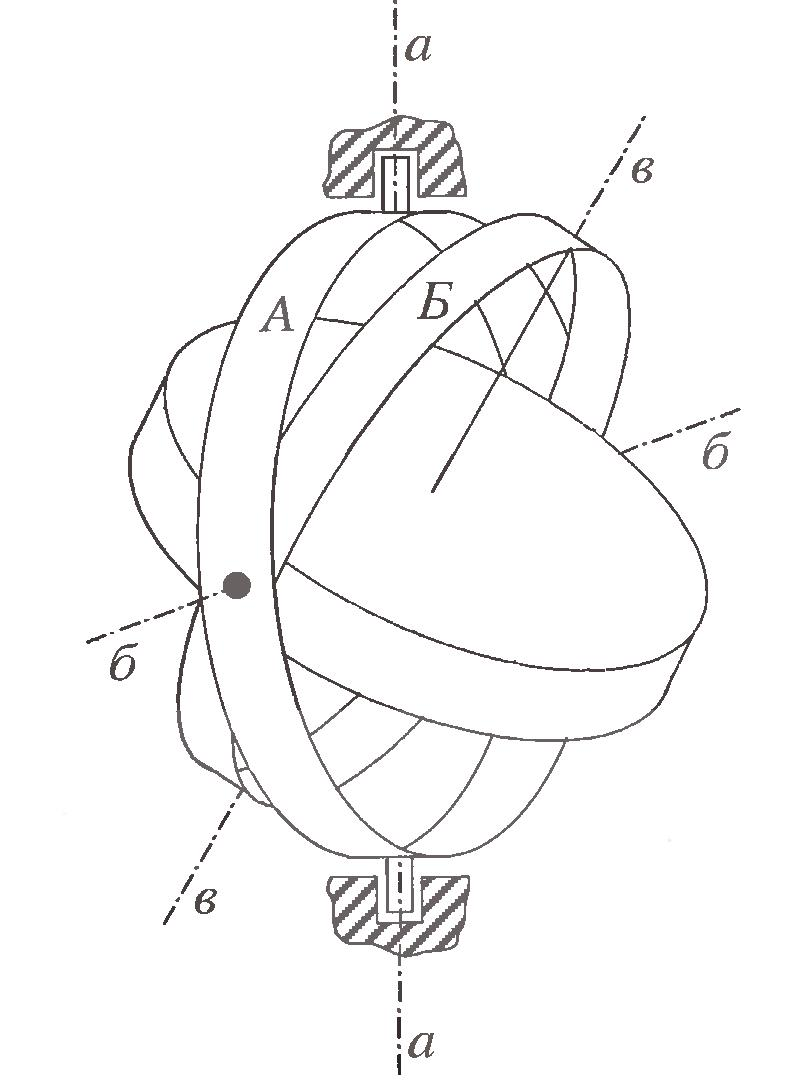
\includegraphics[width=0.29\linewidth]{Cardan_suspension} 	
			\label{fig:Cardan_suspension}}
	\subfigure[]{
		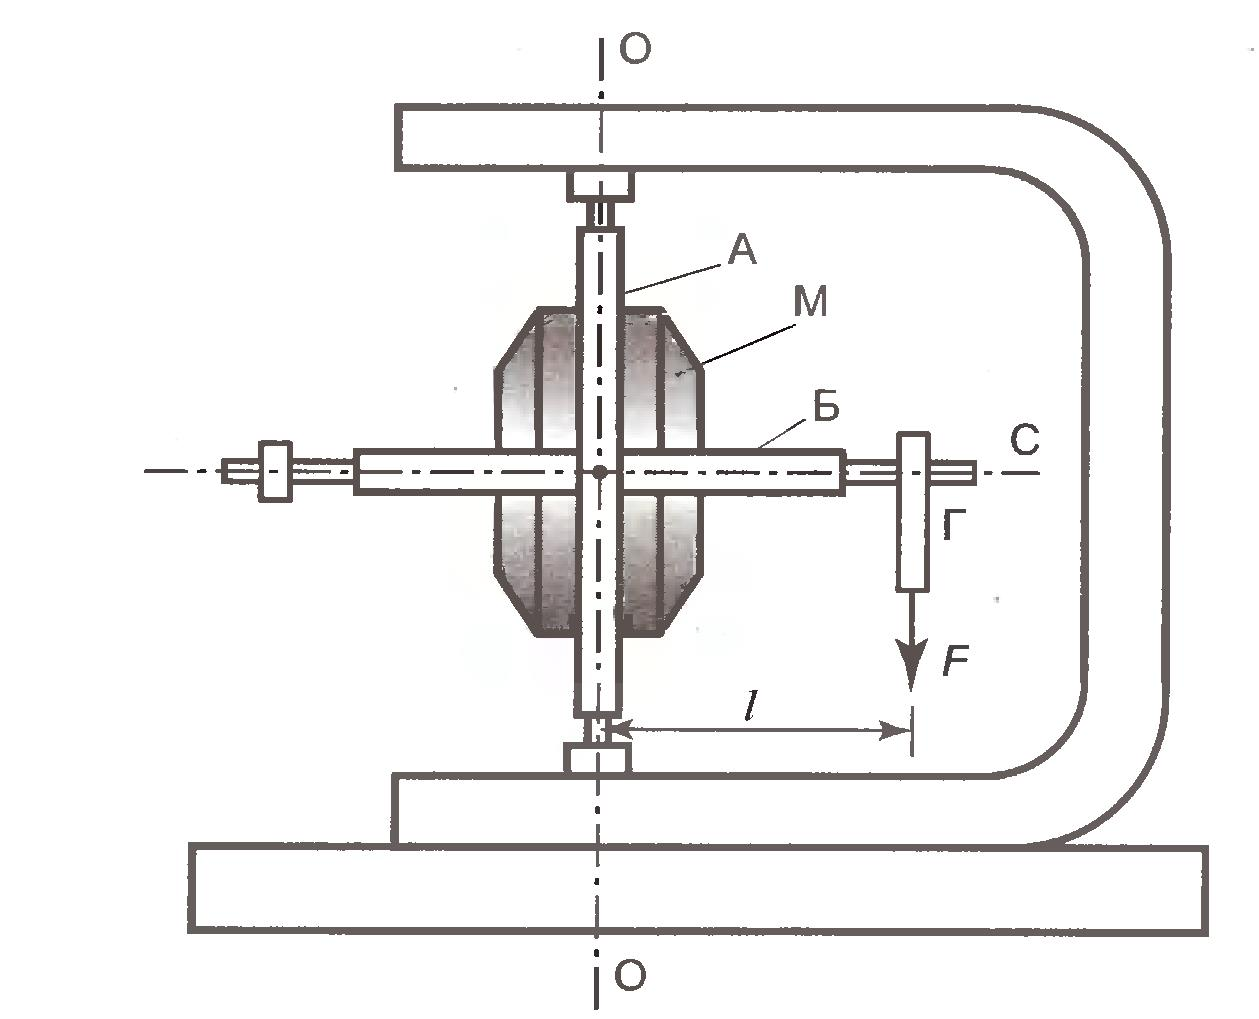
\includegraphics[width=0.45\linewidth]{facility} 
			\label{fig:facility} }  
	\caption{(а) Гироскоп, закрепленный в карданном подвесе, (б) Схема устройства гироскопа.}
\end{figure}

Ротором гироскопа (Рис. \ref{fig:facility}) является ротор электромотора М. Кожух мотора скреплен с кольцом Б (Рис. \ref{fig:Cardan_suspension}). Мотор с кольцом Б может вращаться в кольце А вокруг горизонтальной оси бб, которое может вращаться относительно оси аа. Рычаг С направлен по оси симметрии ротора. на рычаг подвешивают грузы Г.

Измерение скорости прецессии гироскопа позволяет вычислить угловую скорость вращения его ротора. Расчет производится по формуле (8). Момент инерции ротора относительно оси симметрии $I_0$ пизмеряется по крутильным колебаниям точной копии ротора, подвешиваемой вдоль оси симметриии наж есткой проволоке. Период крутильных колебаний $T_0$ зависит от момента инерции $I_0$ и модуля кручения проволоки $f$:
\[T_0 = 2\pi \sqrt{\frac{I_0}{f}}. \]

Чтобы исключить модуль кручения проволоки, вместо ротора гироскопа к той же проволоке подвешивабт цилиндр правильной форму с известным размерами и массов, для которого легко можно вычислить момент инерции $I_{\text{ц}}$. Для определения момента инерции ротора гироскопа имее \[ I_0 = I_{\text{ц}}\frac{T_0^2}{T_{\text{ц}}^2}, \]
здесь $I_{\text{ц}}$ -- период крутильным колебаний цилиндра.

Также частоту вращения ротора можно определить по фигурам Лиссажу.

\subsection*{Ход работы}
Сперва определим погрешности приборов:
\begin{itemize}
	\item линейка: $2\cdot\dfrac{\text{цена деления}}{2} = 1$ мм
	\item секундомер: с учетом реакции человека $0.5$ с
	\item электронные весы: $1$ г
\end{itemize}
\begin{enumerate}
	\item Устанавливаем ось гироскопа в горизонтальное положение, осторожно поворачивая ее за рычаг $C$.
	\item Включаем питание гироскопа и ждем 4-5 минут, чтобы вращение ротора успело стабилизироваться.
	\item Убеждаемся в том, что ротом вращается достаточно быстро: при легком постукивании по рычагу $C$ последний не должен изменят ьсвоего положения в пространтсве. <<Поиграемся>> с гироском, нажимая карандашом на рычаг $C$. По реакции гороскопа определяем в какую сторону вращается ротора.
	\item Подвесим к рычагу $C$ груз $\text{Г}$. При этом должна начаться прецессия гироскопа. Трение в оси приводит к тому, что рычаг $C$ начинает медленно опускаться.
	\item Отклоняем рычаг $C$ на $5-6$ градусов вверх от горизонтальной плоскости. Подвесим к нему груз $\text{Г}$ и с помощью секундомера найдем угловую скорость регулярной прецесси $\Omega$, находить ее будем по числу оборотов и времени прецессии. Измерения продолжаем до тех пор, пока рычаг $C$  не опустится на $5-6$ градусов ниже горизонтальной плоскости, сделав целов число оборотов относительно вертикальной оси. Измеряем также скорость опускания рычага $C$. Повторять опыт будем не менее пяти раз. В конце усредним результаты.
	$$
		T = \frac{t_{\text{полн}}}{N}
	$$
	
	$$
		\Omega = \frac{2\pi N}{t_{\text{полн}}}
	$$
	\begin{table}[h]
		\centering
		\begin{tabular}{|c|c|c|c|c|c|c|c|c|} \hline
			№ опыта & $m$, г & $N$ & $t$, с  & $T$, с  & $h_0$, см & $h_{\text{к}}$, см & $\Omega$, с$^{-1}$ & $v,~^{\circ}$/с	  \\ \hline
			$1$ 	& $329$  & $4$ & $122.2$ & $30.55$ & $17.8$    & $15.5$ 			& $0.206$ 			 & $0.082$		  	  \\ \hline
			$2$ 	& $329$  & $4$ & $122.3$ & $30.58$ & $17.6$	   & $15.8$				& $0.206$ 			 & $0.082$		  	  \\ \hline
			$3$ 	& $329$  & $4$ & $122.6$ & $30.65$ & $17.7$    & $15.4$ 			& $0.205$ 			 & $0.082$		  	  \\ \hline
			$4$ 	& $329$  & $4$ & $122.8$ & $30.70$ & $17.7$	   & $15.1$ 			& $0.205$ 			 & $0.081$		  	  \\ \hline
			$5$ 	& $329$  & $4$ & $122.8$ & $30.70$ & $17.8$	   & $15.3$				& $0.205$ 			 & $0.081$		  	  \\ \hline
		\end{tabular}
		\caption{Первый опыт}
		\label{tab:first}
	\end{table}
	Усредним значения:
	$$
	\Omega = 205.4~\text{с$^{-1}$}
	$$
	$$
	v = 0.392^{\circ}/\text{с}
	$$
	\item Проделаем всю серию экспериментов, описаннных в пункте 5 при $5-7$ значениях момента $M$ силы $F$ относительно центра масс гироскопа (длина плеча $l = 12.1\pm 0.1$ см). Результаты опытов занесем в таблицу \ref{tab:6} и изобразим в виде графика $\Omega$ в зависимости от $M$. 
	\begin{table}[h]
		\centering
		\begin{tabular}{|c|c|c|c|c|c|c|c|c|} \hline
			№ опыта & $m$, г & $N$ & $t$, с & $T$, с & $h_0$, см & $h_{\text{к}}$, см & $\Omega$, Гц & $M$, Н$\cdot$м \\ \hline
			$1$ & $329$ & $4$ & $122.6$ & $30.65$ & $17.7$ & $15.4$ & $0.205$ & $0.391$ \\ \hline
			$2$ & $329$ & $4$ & $122.8$ & $30.70$ & $17.7$ & $15.1$ & $0.205$ & $0.391$ \\ \hline
			$3$ & $329$ & $4$ & $122.8$ & $30.70$ & $17.8$ & $15.3$ & $0.205$ & $0.391$ \\ \hline
			$4$ & $271$ & $3$ & $111.8$ & $37.27$ & $15.7$ & $15.7$ & $0.169$ & $0.322$ \\ \hline
			$5$ & $271$ & $3$ & $111.9$ & $37.30$ & $15.6$ & $15.6$ & $0.168$ & $0.322$ \\ \hline
			$6$ & $271$ & $3$ & $111.8$ & $37.27$ & $15.7$ & $15.7$ & $0.169$ & $0.322$ \\ \hline
			$7$ & $218$ & $3$ & $138.7$ & $46.23$ & $15.2$ & $15.2$ & $0.136$ & $0.259$ \\ \hline
			$8$ & $218$ & $3$ & $138.2$ & $46.07$ & $15.4$ & $15.4$ & $0.136$ & $0.259$ \\ \hline
			$9$ & $218$ & $3$ & $138.6$ & $46.20$ & $15.4$ & $15.4$ & $0.136$ & $0.259$ \\ \hline
			$10$ & $174$ & $2$ & $114.6$ & $57.30$ & $15.8$ & $15.8$ & $0.110$ & $0.207$ \\ \hline
			$11$ & $174$ & $2$ & $114.6$ & $57.30$ & $15.6$ & $15.6$ & $0.110$ & $0.207$ \\ \hline
			$12$ & $174$ & $2$ & $115.1$ & $57.55$ & $15.7$ & $15.7$ & $0.109$ & $0.207$ \\ \hline
			$13$ & $142$ & $2$ & $142.7$ & $71.35$ & $15.6$ & $15.6$ & $0.088$ & $0.169$ \\ \hline
			$14$ & $142$ & $2$ & $142.4$ & $71.20$ & $15.5$ & $15.5$ & $0.088$ & $0.169$ \\ \hline
			$15$ & $142$ & $2$ & $142.8$ & $71.40$ & $15.5$ & $15.5$ & $0.088$ & $0.169$ \\ \hline
			$16$ & $116$ & $2$ & $175.6$ & $87.80$ & $15.4$ & $15.4$ & $0.072$ & $0.138$ \\ \hline
			$17$ & $116$ & $2$ & $175.5$ & $87.75$ & $15.4$ & $15.4$ & $0.072$ & $0.138$ \\ \hline
			$18$ & $116$ & $2$ & $175.7$ & $87.85$ & $15.2$ & $15.2$ & $0.071$ & $0.138$ \\ \hline
		\end{tabular}
		\caption{Опредление моментов силы $M$ и угловой скорости $\Omega$ для различных $m$}
		\label{tab:6}
	\end{table}

	Момент силы $M$ здесь находится по формуле
	$$
	M = mgl
	$$
	\begin{figure}[h!]
		\centering
		\begin{tikzpicture}[dot/.style = {draw, fill = black, color = black, circle, inner sep=1.5pt}, >=stealth]
			\begin{axis}
				[
				width = 0.68\paperwidth, 
				xlabel = {$\Omega$, с$^{-1}$}, 
				ylabel = {$M$, Н$\cdot$м}, 
				%grid=both, 
				ymin = 0.051, ymax = 0.2,
				xmin = 0.1, %xmax = 70,
				xtick={0.1,0.2,...,0.4},
				ytick={0.1,0.15,0.2},
				]
				
				\addplot+[black,only marks,mark = *,
				mark options = {
					scale = 1.0, 
					fill = black
				}] coordinates {(0.391, 0.205) (0.322, 0.169) (0.259, 0.136) (0.207, 0.110) (0.169, 0.088) (0.138, 0.072)};
				\addplot[black, domain=0.1:0.4] {0.5252 * x};
			\end{axis}
		\end{tikzpicture}
		\caption{График зависимости $M$ от $\Omega$}
		\label{graph1}
	\end{figure}

	Из формулы (\ref{eq:teor_equation_omega})
	$$
	\frac{mgl}{I_z\omega_0}~\Rightarrow~\omega_0\propto\frac{M}{\Omega} = k
	$$

	Методом наименьших квадратов определим коэффициенты построенной зависимости.
	$$
	k = \frac{<x y> - <x> <y>}{<x^2> - {<x>}^2} = 0.525~\frac{\text{Н$\cdot$м}}{\text{с$^{-1}$}}
	$$
	$$
	b = <y> - k<x> \approx 0
	$$
	Величина $b$ близка к нулю, что согласуется с теорией.

	Погрешность коэффициента $k$:
	$$
	{\sigma_k}^{\text{сл}}= \sqrt{\frac{1}{n-2}\left(\frac{D_{yy}}{D_{xx}} - k^2 \right)} = 0.017~\frac{\text{Н$\cdot$м}}{\text{с$^{-1}$}}
	$$
	Получим
	$$
	k = 0.525\pm 0.017~\frac{\text{Н$\cdot$м}}{\text{с$^{-1}$}}
	$$
	\item Измеряем момент инерции ротора гироскопа относительно оси симметрии $I_0$. Для этого подвесим ротор, извлеченный из такого же гироскопа, к концу вертикально висящей проволоки так, чтобы ось симметрии гироскопа была вертикальна, и измеряем период крутильных колебаний получившегося маятника. Далее заменяем ротом гироскопа цилиндром, для которого известны или легко могут быть измерены радиус и масса, и определяем для него период крутильных колебаний. Пользуясь формулой (10) вычисляем момент инерции ротора гироскора $I_0$.

	Измерим размеры цилиндра: $m = 1616.9 \pm 0.1 \text{г}, d = 78.1 \pm 0.1 \text{мм}$ 
	
	Момент инерции для цилиндра:
	$$
	I_{\text{ц}} = \frac{md^2}{8} = 1.23\cdot10^{-3}~\text{кг$\cdot$м$^2$}
	$$
	$$
	\sigma_{I_{\text{ц}}} = \sqrt{\left(\frac{\partial{I}}{\partial{m}}\right)^2\cdot\sigma_m^2 + \left(\frac{\partial{I}}{\partial{d}}\right)^2\cdot \sigma_d^2} \approx 0
	$$
	Измерим периоды колебаний цилиндра и ротора:
	$$
	T_{\text{ц}} = 4.05\pm 0.02~\text{c}
	$$
	$$
	T_{\text{р}} = 3.21\pm 0.02~\text{c}
	$$
	$$
	I_{\text{р}}= I_{\text{ц}}\frac{T_{\text{р}}^2}{{T_{\text{ц}}}^2} = 0.77\cdot10^{-3}~\text{кг$\cdot$м$^2$}
	$$

	\item
	
	Погрешность $I_{\text{р}}$:
	$$
	\sigma_{I_{\text{р}}} = \sqrt{\left(\frac{\partial{I}}{\partial{I_{\text{ц}}}}\right)^2\cdot\sigma_{I_{\text{ц}}}^2 + \left(\frac{\partial{I}}{\partial{T_{\text{ц}}}}\right)^2\cdot \sigma_{T_{\text{ц}}}^2 + \left(\frac{\partial{I}}{\partial{T_{\text{р}}}}\right)^2\cdot \sigma_{T_{\text{р}}}^2} = 0.02\cdot 10^{-3}~\text{кг$\cdot$м$^2$}
	$$
	$$
	I_{\text{р}} = (0.77\pm 0.02)\cdot 10^{-3}~\text{кг$\cdot$м$^2$}
	$$
	Полная погрешность величины $\Omega$ пределяется из ее приборной и случайной погрешности.
	$$
	\sigma_{\text{случ}} = \sqrt{\frac{1}{N(N-1)}\sum_{i = 1}^{N} (\Omega_i - \overline{\Omega})^2},~\sigma_{\text{пр}} = \frac{\sigma_t}{N}
	$$
	$$
	\sigma_{\Omega} = \sqrt{\sigma_{\text{случ}}^2 + \sigma_{\text{пр}}^2}\approx 0.001~\text{Гц}
	$$

	\item
	Далее найдем частоту вращения ротора:
	$$
	\omega = 2\pi\nu = \frac{L}{I_{\text{р}}}~\Rightarrow~\nu = \frac{L}{2\pi I_{\text{р}}} = \frac{1}{2\pi I_{\text{р}}\dfrac{1}{L}} = \frac{1}{2\pi I_{\text{р}} k}
	$$
	$$
	\nu = 394~\text{Гц}
	$$
	Погрешность величины $\nu$:
	$$
	\sigma_{\nu} = \sqrt{\left(\frac{\partial{\nu}}{\partial{I_{\text{р}}}}\right)^2\cdot\sigma_{I_{\text{р}}}^2 + \left(\frac{\partial{\nu}}{\partial{k}}\right)^2\cdot \sigma_k^2} = 16~\text{Гц}
	$$
	Итого
	$$
	\nu = 394\pm 16~\text{Гц}
	$$

	\item
	Измерим теперь момент силы трения в оси, перпендикулярной оси вращения:
	$$
	M = \frac{2L\alpha}{t} = \frac{2\alpha}{tk}
	$$
	В нашем случае $\alpha = 5^{\circ}$

	Определим для каждого груза:
	\begin{table}[h]
		\centering
		\begin{tabular}{|c|c|c|c|} \hline
			№ груза & $m$, г & $t$, с & $M_{\text{тр}}$, $10^{-3}$ Н$\cdot$м  \\ \hline
			$1$ & $329$ 	 & $122.6$ & $2.72\pm 0.05$ \\ \hline
			$2$ & $271$ 	 & $111.8$ & $2.97\pm 0.05$ \\ \hline
			$3$ & $218$ 	 & $138.7$ & $2.40\pm 0.04$ \\ \hline
			$4$ & $174$ 	 & $114.6$ & $2.90\pm 0.05$ \\ \hline
			$5$ & $142$ 	 & $142.7$ & $2.33\pm 0.04$ \\ \hline
			$6$ & $116$ 	 & $175.6$ & $1.89\pm 0.03$ \\ \hline
		\end{tabular}
		\caption{Опредление моментов силы трения для различных $m$}
		\label{tab:10}
	\end{table}

	Усредненное значение:
	$$
	M_{\text{тр}} = 2.54\cdot 10^{-3}~\text{Н$\cdot$м}
	$$
	Приборная погрешность
	$$
	\sigma_{\nu} = \sqrt{\left(\frac{\partial{M_{\text{тр}}}}{\partial{t}}\right)^2\cdot\sigma_{t}^2 + \left(\frac{\partial{M_{\text{тр}}}}{\partial{k}}\right)^2\cdot \sigma_k^2}
	$$

	\item

	Определим теперь частоту вращения гироскопа с помощью осциллографа и фигур Лиссажу: для этого подключим гироскоп к осциллографу. Из эксперимента $\nu\approx 400$ Гц значит выставляем на осциллографе частоту $360$ Гц, отключаем питание ротора гироскопа (и более ничего с ним не делаем в ходе этих измерений), и смотрим на экран осциллографа. Когда на нем будет остановившийся эллипс, это значит, что частота вращения гироскопа совпадает с частотой выдаваемой осциллографом, а значит частота вращения гироскопа уменьшилась до $380$ Гц. Как можно быстрее переключаем частоту осциллографа на 360 и повторяем вышеизложенные действия. Для каждой частоты засекаем время от отключения гироскопа до совпадения частоты вращения гироскопа и частоты осциллографа. Делаем так для $10$ частот. Результаты заносим в таблицу:
	\begin{table}[h]
		\centering
		\begin{tabular}{|c|c|c|} \hline
			№ опыта & $\nu$, Гц & $t$, с \\ \hline
			$1$ & $360$ & $77.7$  \\ \hline
			$2$ & $340$ & $134.2$ \\ \hline
			$3$ & $320$ & $192.2$ \\ \hline
			$4$ & $300$ & $257.8$ \\ \hline
			$5$ & $280$ & $313.3$ \\ \hline
			$6$ & $260$ & $376.9$ \\ \hline
			$7$ & $240$ & $446.3$ \\ \hline
			$8$ & $220$ & $519.6$ \\ \hline
			$9$ & $200$ & $597.2$ \\ \hline
			$10$ & $180$ & $680.6$ \\ \hline
		\end{tabular}
		\caption{Опыт с осциллографом}
		\label{tab:11}
	\end{table}
	Построим график $\nu(t)$.
	\begin{figure}[h!]
		\centering
		\begin{tikzpicture}[dot/.style = {draw, fill = black, color = black, circle, inner sep=1.5pt}, >=stealth]
			\begin{axis}
				[
				width = 0.68\paperwidth, 
				xlabel = {$t$, с}, 
				ylabel = {$\nu$, Гц}, 
				grid=both, 
				%ymin = 0.051, ymax = 0.2,
				%xmin = 0.1, %xmax = 70,
				%xtick={0.1,0.2,...,0.4},
				%ytick={0.1,0.15,0.2},
				]
				
				\addplot+[black,only marks,mark = *,
				mark options = {
					scale = 1.0, 
					fill = black
				}] coordinates {(77.7, 360) (132.2, 340) (192.2, 320) (257.8, 300) (313.3, 280) (376.9, 260) (446.3, 240) (519.6, 220) (597.2, 200) (680.6, 180)};
				%\addplot[black, domain=0.1:0.4] {0.5252 * x};
			\end{axis}
		\end{tikzpicture}
		\caption{График зависимости $\nu$ от $t$}
		\label{graph2}
	\end{figure}

	Методом наименьших квадратов определим коэффициенты построенной зависимости.
	$$
	k = \frac{<x y> - <x> <y>}{<x^2> - {<x>}^2} = -0.301~1/\text{с}^2
	$$
	$$
	b = <y> - k<x> = 378.0~\text{Гц}
	$$

	\item
	Погрешность коэффициента $k$:
	$$
	{\sigma_k}^{\text{сл}}= \sqrt{\frac{1}{n-2}\left(\frac{D_{yy}}{D_{xx}} - k^2 \right)} = 0.004~1/\text{с}^2
	$$
	Коэффициента $b$:
	$$
	\sigma_b = \sigma_k \sqrt{<x^2> - <x>^2}\approx 1~\text{Гц}
	$$
	Приборные погрешности:
	$$
	\sigma_k^{\text{пр}} = \sigma_t \approx 0,~\sigma_b = \sigma_t = 0.5
	$$
	Итого
	$$
	k = -0.301\pm 0.004~1/\text{с}^2,~b = 378.0\pm 1.2~\text{Гц}
	$$
	Частоты вращения ротора, найденные в пунктах 9 и 11 совпадают в пределах погрешности.

	\item 
	Применимость $L_{\Omega} << L_{\omega_0}$ верна из-за отношения угловых скоростей: $\Omega \approx 10^{-3}$ Гц, в то время как $\omega_0 \approx 2550$ Гц.

	\item Используя коэффициент $k$ можно найти момент силы трения в оси, параллельной оси вращения гироскопа:
	$$
	\frac{dL}{dt} = -M~\Rightarrow~dL = d(I_{\text{р}}\omega) = I_{\text{р}}\cdot d\omega = 2\pi I_{\text{р}} d\nu
	$$
	Тогда
	$$
	M = -2\pi I_{\text{р}} \frac{d\nu}{dt}
	$$
	А в нашем случае 
	$$
	\frac{d\nu}{dt} = k~\Rightarrow~M = -2\pi I_{\text{р}}k = 1.46 \cdot 10^{-3}~\text{Н}\cdot\text{м}
	$$
	Погрешность равна
	$$
	\sigma_M = \sqrt{I_{\text{р}}^2\cdot\sigma_k + k^2\cdot\sigma_{I_{\text{р}}}} = 0.01 \cdot 10^{-3}~\text{Н}\cdot\text{м}
	$$
	Итого:
	$$
	M = (1.46 \pm 0.01) \cdot 10^{-3}~\text{Н}\cdot\text{м}
	$$
\end{enumerate}

\textbf{Вывод}
\begin{itemize}
	\item В ходе выполнения работы были определены физические величины, описывающие регулярную прецессию гироскопа, а именно:
		\begin{itemize}
			\item Была определена теоретически и экспериментально угловая скорость регулярной прецессии гироскопа. Полученная точность теоретически определенной величины совпадает с точностью, с которой можно определить момент инерции ротора гироскопа, так как эта величина вносит наибольший вклад в погрешность.
			\item Был определен момент инерции ротора гироскопа. Основной вклад -- погрешность измерения радиуса цилиндра, с помощью которого определялась данная величина.
			\item Был определен момент сил трения, возникающих в оси, перпендикулярной оси вращения. Основной вклад.
		\end{itemize}
	\item На практике были подтверждены все теоретические зависимости, используемые в данной работе.
	\item Показано соответствие различных методов определения физических величин: угловая скорость, частота.
	\item Достигнута приемлемая точность.
\end{itemize}



\end{document}


